Für die Sektion der Beispiele werden sich primär Klassiker angeschaut, welche als Grundlage und Überblick des Genres dienen sollen.
Als Klassiker werden im folgenden Spiele genannt, welche bereits etwas älter sind, und maßgeblich beteiligt waren an der Bildung und Entwicklung dieses Genres. Vorwiegend haben die genannten Spiele also großen Anklang in der Community gefunden und wurden sehr gut aufgenommen. Der Zeitraum beschränkt sich folgend auf die Jahre 1980 - 2010. Die genannten Spiele sind dabei lediglich ein Ausschnitt aller vorhandenen Klassiker und Meilensteine des Genres. Ein weiteres Beispiel eines Resource Management Games, welches erst kürzlich (2018) erschien, wird in der folgenden Sektion \textit{Analyse} genauer untersucht und dabei maßgeblich für die Entwicklung des Prototypen sein.

\subsection{Age of Empires}
Das Spiel \textit{Age of Empires} ist ein von \textit{Ensemble Studios} entwickeltes und von \textit{Microsoft} publiziertes, historisches Echt-Zeit-Strategie-Spiel für Einzel- und Mehrspieler, welches in Amerika im Jahr 1997 erschien. Die verwendete \textit{game engine} ist \textit{Genie}, welche hauptsächlich 2D \textit{sprites} verwendet \cite{aoe}. Age of Empires ist dabei der erste Teil der Reihe, mit drei weiteren Nachfolgern \textit{Age of Empires II, Age of Empires III} und \textit{Age of Empires IV}, und einem Ableger mit mythologischem Hintergrund \textit{Age of Mythology} \cite{aoe2}. Das Spiel wird in einer isometrischen Perspektive dargestellt (vgl. \autoref{image:aoe}). Es gibt verschiedenste Ressourcen und Einheiten, welche verschiedene Taktiken ermöglichen mit wiederum verschiedenen Konterstrategien. Ressourcen sind dabei finit, was bedeutet, dass ein gefällter Baum nicht wieder nachwachsen wird. Eine Kernkomponente des Spiels sind die verschiedenen Zeitalter, in welche der Spieler voranschreiten kann. Damit werden jeweils neue Technologien und Einheiten freigeschaltet, welche auf dem Weg zum Sieg hilfreich sein könnten. Die Zeitalter gliedern sich dabei auf in \textit{Altsteinzeit}, \textit{Jungsteinzeit}, \textit{Bronzezeit} und \textit{Eisenzeit} \cite*[]{aoe}. Es gibt dabei 12 verschiedene Völker, die an historische Völker angelehnt sind. Diese sind \textit{Ägypter, Assyrer, Babylonier, Chosonen, Griechen, Hethiter, Minoer, Perser, Phönizier, Shang, Sumerer} und \textit{Yamato}. Dabei hat jedes Volk eine andere Gesamtauswahl aus dem Technologiebaum. Alle wichtigen Eckdaten zu dem Spiel sind in \autoref{table:aoe} einsehbar.
\paragraph*{Siegbedingungen}
\begin{itemize}
    \item Alle Gegenspieler eliminieren mittels Militär
    \item Alle \textit{Artefakte} / Runen erobern
    \item Ein \textit{Weltwunder} bauen und erfolgreich bis Ende verteidigen
\end{itemize}

\paragraph*{Ressourcen}
\begin{itemize}
    \item Nahrung
    \item Holz
    \item Stein
    \item Gold
\end{itemize}\cite*[]{aoe:ressources}
\newparagraph{Rezensionen}
\begin{tabularx}{0.8\textwidth} { 
    | >{\raggedright\arraybackslash}X 
    | >{\centering\arraybackslash}X 
    | >{\raggedleft\arraybackslash}X | }
   \hline
   PC Games & 93\% \cite*[]{aoepcgames}\\
   \hline
   PC Player & 5/5 \cite*[]{aoepcplayer}\\
  \hline
  Power Play & 84\% \cite*[]{aoepowerplay}\\
  \hline
  GameRankings & 87,1\% \cite*[]{aoegamerankings}\\
  \hline
  IGDB & 85\% \cite*[]{aoe}\\
  \hline
\end{tabularx}

\begin{table}[]
    \centering
    \caption{Age of Empires Eigenschaften (\cite*[]{aoe,aoe:ressources,aoe2, aoe:technologies})}
    \label{table:aoe}
    \begin{tabular}{|l|l|}
    \hline
    Erscheinungsjahr & 1997                              \\ \hline
    Entwickler       & Ensemble Studios                  \\ \hline
    Publisher        & Microsoft                         \\ \hline
    Multiplayer        & Ja                         \\ \hline
    Ressourcen       & Nahrung, Holz, Stein, Gold        \\ \hline
    Siegbedingungen  & Domination, Artefakte, Weltwunder \\ \hline
    Spielbare Völker & 12                                \\ \hline
    Perspektive      & Isometrisch                       \\ \hline
    Technologien     & 53                                \\ \hline
    \end{tabular}
    \end{table}


\begin{figure}
    \begin{center}
        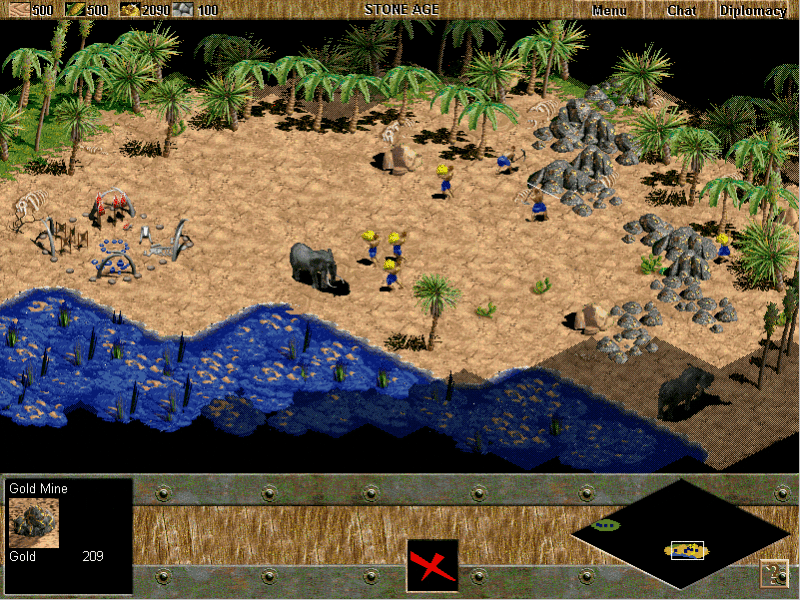
\includegraphics[width=300px]{0.bilder/aoe.png}
    \end{center}
    \caption{Screenshot aus Age of Empires (\cite{aoe})} \label{image:aoe}
\end{figure}
\subsection{Sid Meier's Civilization}
Das 1991 erschienene Spiel \textit{Sid Meier's Civilization} ist ein von \textit{MicroPose} entwickeltes und publiziertes, rundenbasiertes Strategiespiel \cite*[]{civigdb}. \textit{MicroPose} ist ein 1982 von Bill Stealey und Sid Meier gegründetes Softwareunternehmen, wovon von letzterem auch der Name abgeleitet wird \cite*[]{civhistory}. Man startet im Jahr 4000 B.C. und bewegt sich zeitlich bis ins Informationszeitalter, während man neue Städte gründet, Technologien erforscht und anderen Gegenspielern beziehungsweise Reichen und deren Herrschern begegnet, Diplomatie führt und gegebenenfalls auch Kriege. Unter den spielbaren Herrschern sind unter anderem \textit{Alexander der Große, Napoleon} und \textit{Julius Cäsar}. Das Spiel besitzt einen nicht-linearen Technologiebaum mit den wichtigsten Errungenschaften der Menschheit, darunter das Rad oder Navigation, verschiedene baubare Wunder, zum Beispiel die Pyramiden oder die Große Mauer und besitzt fünf verschiedene Schwierigkeitsgrade, mit denen der Spieler die Herausforderung selber setzen \cite*[]{civ}. Je nach Fokus des Spielers ist also jedes Match ein neues, und es gibt durch verschiedene Ressourcen und Entscheidungsmöglichkeiten einige Strategien denen sich der Spieler bedienen kann. \\
Das Spiel erhielt fünf weitere Nachfolger \textit{Civilization II, Civilization III, Civilization IV, Civilization V} und \textit{Civilization VI} \cite*[]{civall}, wobei sich manche Teile stark von anderen Unterscheiden, etwa in der Perspektive oder der Geometrie des Spielfeldes. So wurde von \textit{Civilization IV} auf \textit{Civilization V} das Spielfeld von einem \textit{Square Grid} auf ein \textit{Hex Grid} umgestellt \cite*[]{civallcompare}. Neben den Nachfolgern gab es einige Ableger, darunter \textit{Sid Meier's Civilization: Beyond Earth}, welches 2014 erschien und zwei Erweiterungen erhielt. Dieser Teil spielt, anders als alle anderen, auf einem fremden Planeten und hat eine Sci-Fi Thematik, statt wie üblich, eine historische \cite*[]{civbe}. Das Spiel besitzt, im Gegensatz zu allen anderen Nachfolgern, noch eine Vogelperspektive, statt wie später, eine isometrische (vgl. \autoref{image:civ}). Außerdem sind auch politische Auswahlmöglichkeiten wie Regierungen, oder religiöse Auswahlmöglichkeiten vorhanden. Die wichtigsten Eigenschaften sind in \autoref{table:civ} zusammengefasst.



\paragraph*{Siegbedingungen}
\begin{itemize}
    \item Alle Gegenspieler eliminieren mittels Militär
    \item Ein Raumschiff bauen und Alpha Centauri als erster erreichen
    \item Überleben bis die Zeit ausgelaufen ist \cite*[]{civwin}
\end{itemize}

\paragraph*{Ressourcen}
\begin{itemize}
    \item Kohle
    \item Fisch
    \item Wild
    \item Wild (Tundra)
    \item Edelsteine
    \item Gold
    \item Pferde
    \item Oasen
    \item Öl
    \item Robben
\end{itemize}\cite*[]{civ:ressources}
\newparagraph{Rezensionen}
\begin{tabularx}{0.8\textwidth} { 
    | >{\raggedright\arraybackslash}X 
    | >{\centering\arraybackslash}X 
    | >{\raggedleft\arraybackslash}X | }
    \hline
    IGDB & 93\% \cite*[]{civigdb}\\
    \hline
    AllGame & 5/5 \cite*[]{civ:review:allgame}\\
    \hline
    Game Informer & 8.5/10 \cite*[]{civ:review:gameinformer}\\
    \hline
    Next Generation & 4/5 \cite*[]{civ:review:nextgeneration}\\
    \hline
\end{tabularx}

\begin{table}[]
    \centering
    \caption{Civilization Eigenschaften (\cite*[]{civallcompare,civigdb,civwin, civ:ressources})}
    \label{table:civ}
    \begin{tabular}{|l|l|}
    \hline
    Erscheinungsjahr & 1991                                                                           \\ \hline
    Entwickler       & MicroPose                                                                      \\ \hline
    Publisher        & MicroPose                                                                      \\ \hline
    Multiplayer      & Nein                                                                      \\ \hline
    Ressourcen       & Kohle, Fisch, Wild, Wild (Tundra), Edelsteine, Gold, Pferde, Oasen, Öl, Robben \\ \hline
    Siegbedingungen  & Domination, Space Race, Time                                                   \\ \hline
    Spielbare Völker & 14                                                                             \\ \hline
    Perspektive      & Vogel                                                                          \\ \hline
    Technologien     & 67                                                                             \\ \hline
    \end{tabular}
\end{table}

\begin{figure}
    \begin{center}
        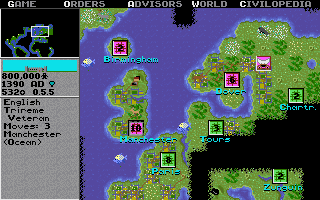
\includegraphics[width=300px]{0.bilder/civ.png}
    \end{center}
    \caption{Screenshot aus Civilization (\cite{civigdb})} \label{image:civ}
\end{figure}
\subsection{Sim City 2000}
Sim City 2000 ist ein im Jahr 1993 erschienenes Städteaufbauspiel für Einzelspieler, welches in das Genre \textit{Simulation} fällt \cite{simcity:ea}. Das Spiel wurde ursprünglich von \textit{Maxis} für den Mac entwickelt und publiziert, wurde in den kommenden Jahren jedoch für weitere Konsolen herausgegeben, darunter \textit{SNES, PlayStation} und \textit{Nintendo 64}. Im Jahr 2005 erschien es schließlich für den PC unter Windows \cite{simcity:igdb}. Der Spieler startet auf einer ausgewählten Karte, welche ein \textit{Square Grid} mit verschiedenen Höhen und Terrain besitzt. Die dabei zentrale Ressource ist Geld in Form von US Dollars. Der Spieler kann mit diesem Geld aus einer breiten Palette an Gebäuden wählen, darunter \textit{Schulen, Bibliotheken, Krankenhäuser} und \textit{Kraftwerke} \cite*[]{simcity:igdb}, welche die Bedürfnisse der Einwohner befriedigen und für Recht und Ordnung in der Stadt sorgen. Diese Gebäude besitzen einen Radius, was ein weiteres strategisches Element dieses Spiels darstellt, da auf möglichst sinnvolles Platzieren der jeweiligen Gebäude geachtet werden muss. Für Wohn-, Industrie- und Kaufhausgebäude markiert der Spieler Zonen, statt die Gebäude einzeln zu setzen. Die Gebäude dieser Zonen werden dann, je nach Bedarf, Stück für Stück aufgebaut oder wieder verlassen. Der Bedarf jeweiliger Zonen ist in \autoref{image:simcity} anhand des grünen (Wohngebäude), des blauen (Kaufhausgebäude) und des gelben (Industriegebäude) Balkens am linken Auswahlbalken erkennbar. Zeigt ein Balken dabei in die Richtung des \textit{+}, so signalisiert das \textit{Bedarf}, zeigt der Balken jedoch in die Richtung des \textit{-}, ist \textit{Überschuss} vorhanden. Zwischen diesen Zonen herrscht eine Relation, so benötigen Kaufhausgebäude die Industriegebäude als Produktionsquelle, und Wohngebäude als Käufer. Die Wohngebäude wiederum benötigen Arbeitsplätze, sowohl in Kaufhausgebäuden als auch in Industriegebäuden. Die Industriegebäude benötigen die Arbeitskräfte der Wohngebäude und Abnehmer für die produzierte Ware in Form von Kaufhausgebäuden. Diese Relation wird wie folgt berechnet (R:C:I beschreibt die Relation zwischen Wohngebäuden zu Kaufhausgebäuden zu Industriegebäuden): 
\newpage
\begin{itemize}
    \item Unter 10.000 Einwohnern: R:C:I = 4:1:3
    \item Zwischen 10.000 und 60.000 Einwohnern: R:C:I = 4:2:2
    \item Über 60.000 Einwohner: R:C:I = 4:3:1 \cite*[]{simcity:somacon}
\end{itemize}
Die Wohngebäude brauchen \textit{Strom, Wasser, Bildung, Sicherheit} und \textit{Freizeitaktivitäten}, welche allesamt durch platzierbare Gebäude gegeben werden können. Bildung ist eine Kernkomponente des Spiels, denn je nach Bildungsgrad der Stadt steigt oder fällt die Kriminalitätsrate und entscheidet auch darüber, welche Industrien blühen oder bankrottgehen. Der Bildungsgrad wird gemessen am EQ (\textit{education quotient}), so erhöht beispielsweise eine Schule den EQ von den 5 bis 20 Jahre alten Bewohnern. Es gibt insgesamt 156 Gebäude, welche in 8 Kategorien eingeteilt werden können, darunter verschiedene Arten von Wohngebäuden, Kaufhausgebäuden oder Industriegebäuden, wie auch verschiedene Parks, Statuen oder Kraftwerke \cite*[]{simcity:fandom}. \\
Ein weiteres zentrales Element des Spiels ist das \textit{Budget}, welche am Ende jedes Spieljahres adjustiert werden kann. So kann man die \textit{Steuern} erhöhen, die die Einwohner zahlen müssen, wie auch die \textit{Ausgaben} für verschiedene Institutionen anpassen. So kann beispielsweise das Budget der Polizei verringert werden oder das Budget der Feuerwehr erhöht werden, woraus jeweils Effektivitätsboni oder -mali folgen \cite*[]{simcity:video}. \\
Das Spiel hat keine Siegbedingungen, die Ziele setzt sich der Spieler selber. Mögliche Ziele sind dabei eine möglichst schöne Stadt, eine Stadt mit möglichst vielen Einwohnern oder man spielt vor sich hin und versucht ein Problem nach dem anderen zu lösen. Auch wenn das Spiel an sich nicht gewonnen werden kann, gibt es dennoch einen Endzustand und eine Art Gewinnsequenz. Der Endzustand ist ein Game Over, bei dem der Spieler durch \$100.000 Dollar Schulden aus \glqq seinem Büro eskortiert wird\grqq, siehe \autoref{image:simcitygameover}. Die mögliche Gewinnsequenz, die einem Sieg am ehesten kommt, ist durch baubare Arkologien bedingt. Arkologien sind sich selbst erhaltende Städte mit einer hohen Bevölkerungsdichte innerhalb eines meist hohen Gebäudes. Der Begriff wurde in den 50er Jahren von dem italienisch-amerikanischen Architekten Paolo Soleri geprägt, jedoch wurde bis heute noch keine echte Arkologie gebaut, auch wenn es dazu bereits einige Experimente, beispielsweise in Arizona, gibt \cite*[]{misc:arcology}. Nachdem der Spieler 301 sogenannte \textit{launch arcos} gebaut hat und das Jahr 2051 bereits angebrochen wurde, erscheint dem Spieler eine Nachricht, in Englisch \textit{\glqq The Exodus has begun\grqq}, woraufhin alle gebauten Arkologien explodieren und dem Spieler suggeriert wird, die Schiffe wären aufgebrochen, um neue Planeten zu besiedeln \cite*[]{simcity:arcology}. \\
Auch wenn das Spiel ein reines \textit{Singleplayer} Game ist, also lediglich ein menschlicher Spieler gleichzeitig spielen kann, spielt man dennoch gegen max. vier weitere Computerspieler, auch genannt \textit{KIs} (Künstliche Intelligenzen). Die maximal vier weiteren angrenzenden Karten der jeweils zu Anfang ausgewählten Karte werden von \textit{KIs} besiedelt und ebenfalls bebaut. Diese Nachbarstädte können mittels gegebener Transportmöglichkeiten, zum Beispiel Flugzeug oder Zug, Gewinn bringen, da die Bewohner der Nachbarstädte in beispielsweise den Kaufhäusern Geld ausgeben \cite*[]{simcity:manual}. \\
Eine weitere Eigenheit des Spiels sind die sogenannten \textit{Katastrophen} beziehungsweise \textit{Desaster}. Diese können vom Spieler komplett ausgeschaltet werden, falls gewollt. Die meisten Desaster können zufällig und natürlich passieren, darunter Feuer, Aufstände oder Fluten. Alle Desaster können ebenfalls vom Spieler selbst initiiert werden, um die Grenzen der eigenen Stadt auf die Probe zu stellen. Manche Katastrophen sind verkettet, so können Aufstände zu Feuer führen, oder Erdbeben zur Explosion von Kernkraftwerken führen, welche wiederum zu Feuern und Aufständen führen kann \cite*[]{simcity:manual}.\\
Das Spiel hatte einen Vorgänger \textit{Sim City}, welcher bereits 1989 erschien, und erhielt neun Nachfolger, darunter \textit{Sim City 3000, Sim City 4} und den neusten Teil \textit{SimCity: BuildIt}, welcher lediglich für mobile Endgeräte verfügbar ist und 2014 erschien. Der letzte Teil für den Computer erschien 2013 und trägt den Titel \textit{SimCity 2013} \cite*[]{simcity:timeline}. \\ Wichtige Eckdaten sind in \autoref{table:simcity} vorzufinden.

\paragraph*{Ressourcen}
\begin{itemize}
    \item Dollar
\end{itemize}
\newparagraph{Rezensionen}
\begin{tabularx}{0.8\textwidth} { 
    | >{\raggedright\arraybackslash}X 
    | >{\centering\arraybackslash}X 
    | >{\raggedleft\arraybackslash}X | }
    \hline
    IGDB & 78\% \cite*[]{simcity:igdb}\\
    \hline
    AllGame & 4.5/5 (PC) \cite*[]{simcity:review:allgame}\\
    \hline
    MacUser & 4.5/5 (Mac) \cite*[]{simcity:review:macuser}\\
    \hline
    Sega Saturn Magazine & 86\% (SAT) \cite*[]{simcity:review:segasaturn}\\
    \hline
\end{tabularx}

\begin{table}[]
    \centering
    \caption{Sim City 2000 Eigenschaften (\cite*[]{simcity:igdb})}
    \label{table:simcity}
    \begin{tabular}{|l|l|}
    \hline
    Erscheinungsjahr & 1993                                                                           \\ \hline
    Entwickler       & Maxis                                                                      \\ \hline
    Publisher        & Maxis                                                                      \\ \hline
    Multiplayer      & Nein                                                                           \\ \hline
    Ressourcen       & Dollars \\ \hline
    Siegbedingungen  & Keine                                               \\ \hline
    Endzustände  & Game Over                                               \\ \hline
    Perspektive      & Isometrisch                                                                          \\ \hline
    \end{tabular}
\end{table}

\begin{figure}
    \begin{center}
        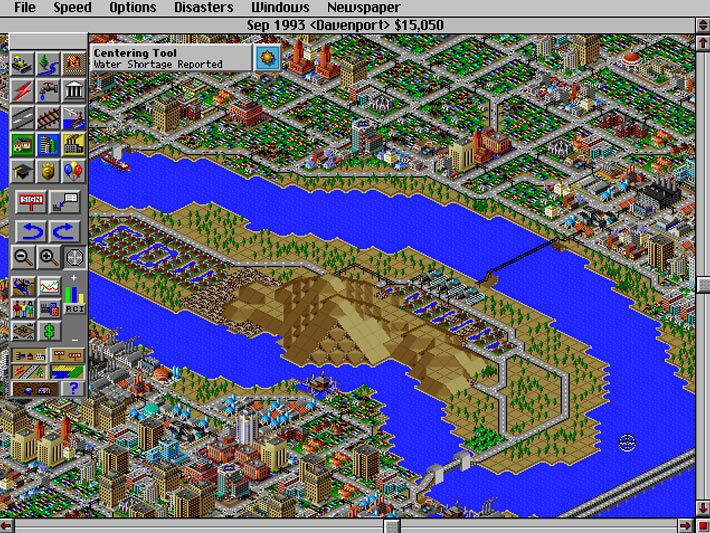
\includegraphics[width=300px]{0.bilder/simcity.jpg}
    \end{center}
    \caption{Screenshot aus Sim City 2000 (\cite{simcity:igdb})} \label{image:simcity}
\end{figure}
\begin{figure}
    \begin{center}
        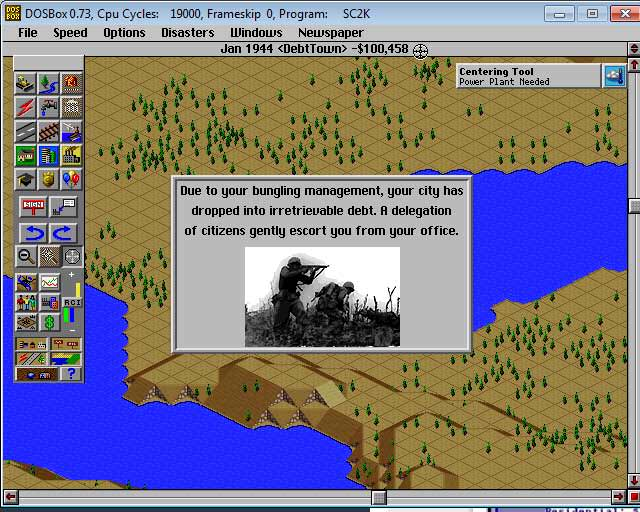
\includegraphics[width=300px]{0.bilder/simcityend.jpeg}
    \end{center}
    \caption{Game Over in Sim City 2000 (\cite{simcity:gameover})} \label{image:simcitygameover}
\end{figure}
\subsection{Weitere Beispiele}
Um den Überblick bestimmter Vertreter des Genres weiter auszubauen, werden im Folgenden weitere interessante Titel genannt, welche eigene Mechaniken innehaben und damit das Genre vorantreiben. Es ist 

\paragraph*{Factorio} Ein im August 2020 erschienenes Strategiespiel, welches von \textit{Wube Software LTD.} entwickelt und publiziert wurde \cite*[]{igdb:factorio} und einen großen Fokus auf Automatisierung und Effizienz legt. Der Spieler beginnt mit dem manuellen Abbau von Ressourcen, und beginnt allmählich primitive Prozesse zu automatisieren mittels Fliesbänder, Öfen und Kisten. Es gibt dabei etliche Produktionsketten mit verschiedenen Tücken und Tricks welche automatisiert werden können und dem Spieler Freiraum für kreatives Denken geben. Nebenbei ist der Spieler der Gefahr von außerirdischen Kreaturen ausgesetzt, welche ab und an angreifen und gegen welche er sich verteidigen muss.

\paragraph*{Frostpunk} Das von \textit{11 bit studios} entwickelte und publizierte Strategiespiel \cite*[]{igdb:frostpunk} fokussiert sich auf das Überleben im Eis. Überlebende Menschen in einer komplett gefrorenen Welt versuchen, eine Stadt zu gründen. Die Tücke dabei ist die Temperatur. Im Kern der Stadt befindet sich ein Generator, welcher stetig mit Kohle betrieben werden muss, da sonst die Menschen der Stadt erfrieren. Ressourcen sind sehr begrenzt und können außerdem über Spähtrupps von der Außenwelt gefunden und zurückgebracht werden, falls diese die Reise überleben. Der Spieler wird immer wieder mit Schneestürmen konfrontiert, welche stetig härter und schwieriger werden. Die Bevölkerung besitzt außerdem ein Level an Moral, welches aufrechterhalten werden muss. Fällt die Moral unter einen gewissen Punkt, endet das Spiel.

\paragraph*{Warcraft III} Veröffentlicht im Jahr 2002, entwickelt und publiziert von \textit{Blizzard Entertainment} \cite*[]{igdb:warcraft}. Das Spiel stellt einen Meilenstein des \textit{Real Time Strategy} Genres dar, wobei man zwischen vier verschiedenen Völkern wählen kann, welche allesamt eigene Einheiten, Eigenschaften und Mechaniken bieten. Außerdem gibt es verschiedene Heldeneinheiten, welche Gegenstände aufsammeln und tragen können und diese damit verstärken.

\paragraph*{Siedler von Catan} Das 1995 erschienene Brettspiel ist bis heute ein gespieltes Gesellschaftsspiel, welches von \textit{Klaus Teuber} entworfen wurde. Das Spielfeld ist in Hexagone aufgeteilt und rundenbasiert, wobei jedes Hexagon einer bestimmten Ressource zugeordnet ist. Die Spieler bauen zwischen den jeweiligen Hexagonen Siedlungen und im Verlauf des Spiels auch Städte, um auf diese Ressourcen Zugriff zu erhalten. 
